\chapter*{perception}
\addcontentsline{toc}{chapter}{perception}
\begin{center}
\vspace{2cm}
\begin{flushright}
\textit{Loud drones, low frequency soothing sounds\\Whispers louder than the loudest screams\\A new detail that changed my day\\The repetitive, unsettling touch\\Tight knots, tight hugs\\Invasive gazes that were not supposed to last\\The faces, the mirrors, the shadows\\Acoustics as the language of every surface}\\
\textbf{M.V.} 
\end{flushright}
\vspace{2cm}
% \vspace*{\fill}
\end{center}
\normalsize

\newpage  % Move to the next page
Self-Organized Criticality describes how certain systems naturally evolve toward a critical, highly sensitive state where small changes can lead to large-scale effects. See figure~\ref{fig:sandpile}. This state of criticality is "self-organized" because the system doesn't require external tuning to reach this point. It naturally arranges itself into this state through its own dynamics. These models help describe the experience of sensory amplification, where the world can be perceived in vivid detail or with overwhelming intensity. \citep{adami1993}

% note: explain my connection to S.O.C.

%% image
\begin{figure}
    \centering
    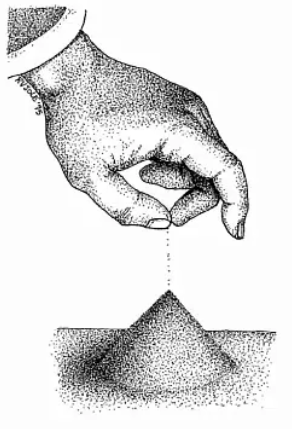
\includegraphics[width=0.8\linewidth]{assets/sandpile.png} 
    \caption{\small Self organized criticality - \textit{Per Bak's Sand pile model, 1988}.}
    \label{fig:sandpile}
\end{figure}

For many, perception unfolds in ways that might differ from conventional understandings. It is often nonlinear and multisensorial, difficult to articulate but deeply felt. The context and balances between anxiety and relaxation shape the sensitivity to sounds and textures. Patterns and structures in an otherwise chaotic environment can be a comforting experience. Time feels non-linear, with moments stretching or compressing, influencing how art and events are experienced.

Immersive or interactive art forms, such as installation art, allow for the direct engagement of multiple senses, mirroring how individuals process the world, translating complex inner experiences into tangible forms. Sensory overload or hyperfocus can transform the relationship between body and world, defining new ways to conceptualize subjectivity.

From a physics standpoint, perception can be understood as a signal processing system, where sensory organs act as transducers, converting energy from one form to another. Interacting photons, wavelengths of a restricted spectrum, pressure variations converted into electrical signals, molecules binding and interacting with receptors, mechanical interactions of skin cells, electromagnetic repulsion, preventing matter from collapsing into itself.

Physics reveals that human perception captures only a small fraction of reality. Neutrinos, dark matter, infrared and ultraviolet light, gravitational waves, and radio signals are imperceptible to us, but part of this reality can be detected with specialized instruments. Can the use of such instruments alter our perception? Is it possible to amplify and alter the ways we relate to the environment by increasing the reach of our perception?

Technology expands our Umwelt by allowing us to access phenomena that are otherwise absent from our perceptual sphere. From infrared imaging to quantum computers, from microscopes to large language models, technology acts as an extension of our perceptual apparatus, expanding our boundaries into previously inaccessible domains.

According to the philosophical approach of post-phenomenology, technology is not neutral. It transforms the nature of perception and experience. Instruments shape what and how we perceive, influencing the object of perception as well as the perceiver.

Our brain is remarkably adaptable and capable of incorporating non-biological sensors into its perceptual framework. This phenomenon is supported by research in neuroscience, cognitive science, and philosophy, particularly in the domains of neuroplasticity, sensory substitution, and embodied cognition. The inclusion of non-biological sensors introduces entirely new dimensions to human perception, effectively expanding the "self."

The extended mind hypothesis, proposed by the philosophers Andy Clark and David Chalmers, argues that tools and technologies can become integral parts of our cognitive processes. Non-biological sensors present in wearable technologies provide continuous streams of data, which the brain learns to process and integrate. This suggests that perception is not confined to the brain and body but extends into the tools we use, fundamentally altering our experience.

If perception relies on external tools, the distinction between "human" and "machine" becomes less clear, leading to a hybridized (cyborg) perception that transcends biology. What counts as "real" if our tools mediate all new experiences? Can the brain adapt to perceive entirely artificial data streams, such as simulations or virtual realities, as seamlessly as it does natural environments?

An overwhelming visual stimulation can sometimes be managed via a calming sound or a specific type of pressure. Since the world is evolving into larger and larger amounts of information and stimuli, it's interesting to wonder if the inclusion of new types of non-biological sensors in our perception will provoke further overstimulation or present opportunities for relaxation based on new calming sensations. Perhaps soon, focusing on calming fluctuations of cosmic microwave background radiation will provide a mental shelter from saturated visual and acoustic inputs in our present environment.
